% !TEX program = pdflatex
% !BIB program = bibtex

% !TEX encoding = UTF-8 Unicode
% !TEX spellcheck = en_us

\documentclass[twoside,twocolumn]{article}

\usepackage[utf8]{inputenc}
\usepackage[english]{babel}

% size for sections and subsections
\usepackage[tiny]{titlesec}
% set the space of sections above and under
\titlespacing{\section}{0pt}{17pt}{4pt}
% set the space of subsections above and under
\titlespacing{\subsection}{0pt}{5pt}{2pt}

% Line spacing
\linespread{1.00}

% reduce space above and under caption in figure
\setlength{\abovecaptionskip}{4pt plus 3pt minus 2pt} 
\setlength{\belowcaptionskip}{-12pt plus 3pt minus 2pt}

% make figure caption smaller
\usepackage{caption}
\captionsetup[figure]{font=footnotesize,labelfont=footnotesize}

% Document margins
\usepackage[hmarginratio=1:1,top=30mm,columnsep=20pt]{geometry}

%tikz
\usepackage{tikz}

\title{\textbf{A Review on Internet of Things (IoT)}}
\author{
    \textsc{Steffen Marbach} \\[0.5ex]
    \normalsize Universität zu Lübeck \\
    \normalsize Lübeck, Germany \\
    \normalsize steffen.marbach@student.uni-luebeck.de \\[1.5ex]
    \normalsize Summary of the work with the same name by M.U. Farooq, Muhammad Waseem, \\
    \normalsize Sadia Mazhar, Anjum Khairi, Talha Kamal \cite{AReViewOnInternetOfThings}
}
\date{}

\begin{document}

\maketitle

\begin{abstract}
   \noindent For now, we communicate either human to human or human to a device. The Internet of Things (IoT) makes a change through machine-to-machine (M2M) communication. This Paper provides a six-layered architecture of IoT and discusses the related key challenges and the associated safety threats.
\end{abstract}

\section{INTRODUCTION}
    \noindent IoT is continually evolving. The opportunities seem infinite. It could provide a global computing network where everything and everyone connects to the Internet. The number of devices availing of internet services is increasing every day. The approach of IoT is converging data obtained from different kinds of things to any virtual platform on existing Internet infrastructure.

    The first IoT device dates back to 1982. A modified coke machine was competent to report the drinks contained and whether the drinks were cold by communicating through the Internet\cite{CokeMachine}.
    
    The basic idea of IoT is to allow an autonomous exchange of valuable information between invisibly embedded different uniquely identifiable real-world devices around us, fueled by the leading technologies like Radio-Frequency Identification (RFID) and Wireless Sensor Networks (WSNs) which are sensed by the sensor devices and further processed for decision making, based on which an automated action is performed.
    
\section{ARCHITECTURE}
    \noindent The existing architecture of the Internet with TCP/ IP protocols cannot handle a network as extensive as IoT. For this issue, there is a need for a new open architecture. This architecture should ensure security and Quality of Service (QoS). Without proper privacy assurance, IoT is not likely to be adopted by many. \cite{ArchitectureIoT} proposed a six-layered architecture divided into the six layers shown in Figure 1. This section will present the six layers of the IoT architecture.
    \subsection{Coding Layer}
        \noindent In this layer, each object gets its unique ID to provide an easy discern \cite{ArchitectureIoT}.        
    \subsection{Perception Layer}
        \noindent This layer consists of data sensors like RFID Tags, IR Sensors, etc. This could sense the temperature, humidity, location, etc. It converts the sensor data into a digital signal and passes it onto the Network Layer for further action.
    \subsection{Network Layer}
        \noindent This layer receives the information as digital signals from the Perception layer and transmits it to the Middleware layer through transmission mediums like WiFi, Bluetooth, 3G, etc. protocols like IPV4, IPV6, etc. are used for this.
    \subsection{Middleware Layer}
        \noindent This layer processes the information provided by the Perception layer through the Network layer. It includes technologies like Cloud computing with direct access to a database to store the data. In some Intelligent Processing Equipment, based on the information a fully automated action is taken based on the processed results of the information.
    \subsection{Application Layer}
        \noindent This layer realizes the applications of IoT With the processed data. The IoT-related applications could be smart homes, transportation, planet, etc.
    \subsection{Business Layer}
        \noindent This layer manages the applications and services of IoT.
    \begin{figure}
        \centering
        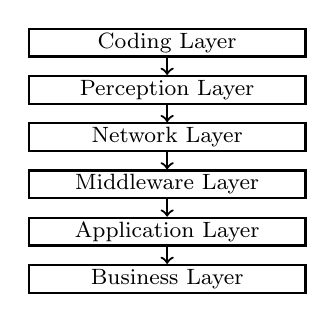
\begin{tikzpicture}
            [node distance={6mm},thick, main/.style = {draw,rectangle,minimum size=10, minimum width=100, inner sep=1pt}] 
            \node[main] (CodingLayer) {\footnotesize Coding Layer};
            \node[main] (PerceptionLayer) [below of=CodingLayer] {\footnotesize Perception Layer};
            \node[main] (NetworkLayer) [below of=PerceptionLayer] {\footnotesize Network Layer};
            \node[main] (MiddlewareLayer) [below of=NetworkLayer] {\footnotesize Middleware Layer};
            \node[main] (ApplicationLayer) [below of=MiddlewareLayer] {\footnotesize Application Layer};
            \node[main] (BusinessLayer) [below of=ApplicationLayer] {\footnotesize Business Layer};
        
            \path[->] (CodingLayer) edge (PerceptionLayer);
            \path[->] (PerceptionLayer) edge (NetworkLayer);
            \path[->] (NetworkLayer) edge (MiddlewareLayer);
            \path[->] (MiddlewareLayer) edge (ApplicationLayer);
            \path[->] (ApplicationLayer) edge (BusinessLayer);
        \end{tikzpicture}
        \caption{Six-Layered Architecture of IoT}
    \end{figure}

\section{APPLICATIONS}
    \noindent Several possible future applications can be of great advantage like smart Hospitals, smart agriculture, smart traffic systems, etc. In this section, we present two of them:
    \subsection{Smart Environment}
        \noindent IoT will predict natural disasters such as floods, fires, earthquakes, etc. Also, there will be proper monitoring of air pollution in the environment.
    \subsection{Smart Home}
        \noindent IoT will provide solutions for Home Automation. We could remotely control our appliances, monitor utility meters, energy, and water supply to help save resources, and build an encroachment detection system that could prevent burglaries. Also, gardening sensors could measure light, humidity, temperature, and other gardening vitals. IoT could water plants according to their needs.

\section{SECURITY AND PRIVACY}
    \noindent IoT makes everything and a person localizable and addressable. So IoT must have a robust security infrastructure. This section will present some of the possible IoT-related issues.
    \subsection{Unauthorized Access to RFID}
        \noindent Unauthorized access to tags is a fundamental issue. Some real-life threats of RFID are RFID Viruses, Side Channel Attacks with a cell phone, and SpeedPass Hack.
    \subsection{ Sensor-Nodes Security Breach}
        \noindent WSNs are vulnerable to attacks because sensor nodes are part of a bi-directional sensor network. \cite{SecurityIssuesWireless} described some of the possible attacks that include Jamming, tampering, Sybil, Flooding, and some other kinds of attacks
    \subsection{Cloud Computing Abuse}
        \noindent The shared resources can face security threats like Man-in-the-middle attacks (MITM), Phishing, etc. The Cloud Security Alliance (CSA) draws attention to hazard like Data Loss, Accounts Hijacking, the Monstrous use of Shared Computers, etc. \cite{SecurityCloudComputing} describes this and other problems closer.
        
\section{CONCLUSION}
    \noindent The IoT is getting bigger and will affect every part of our life. It ranges from automated houses to monitoring health and the environment. We discussed future applications and a six-layered architecture for their use. And the associated safety threats. The development of IoT explains solutions for its security and data protection threats.

    \bibliographystyle{plain}
    {\footnotesize
    \bibliography{Bibliography}}
\end{document}